% !TeX root = ../main.tex
\begin{figure*}[t]
\centering
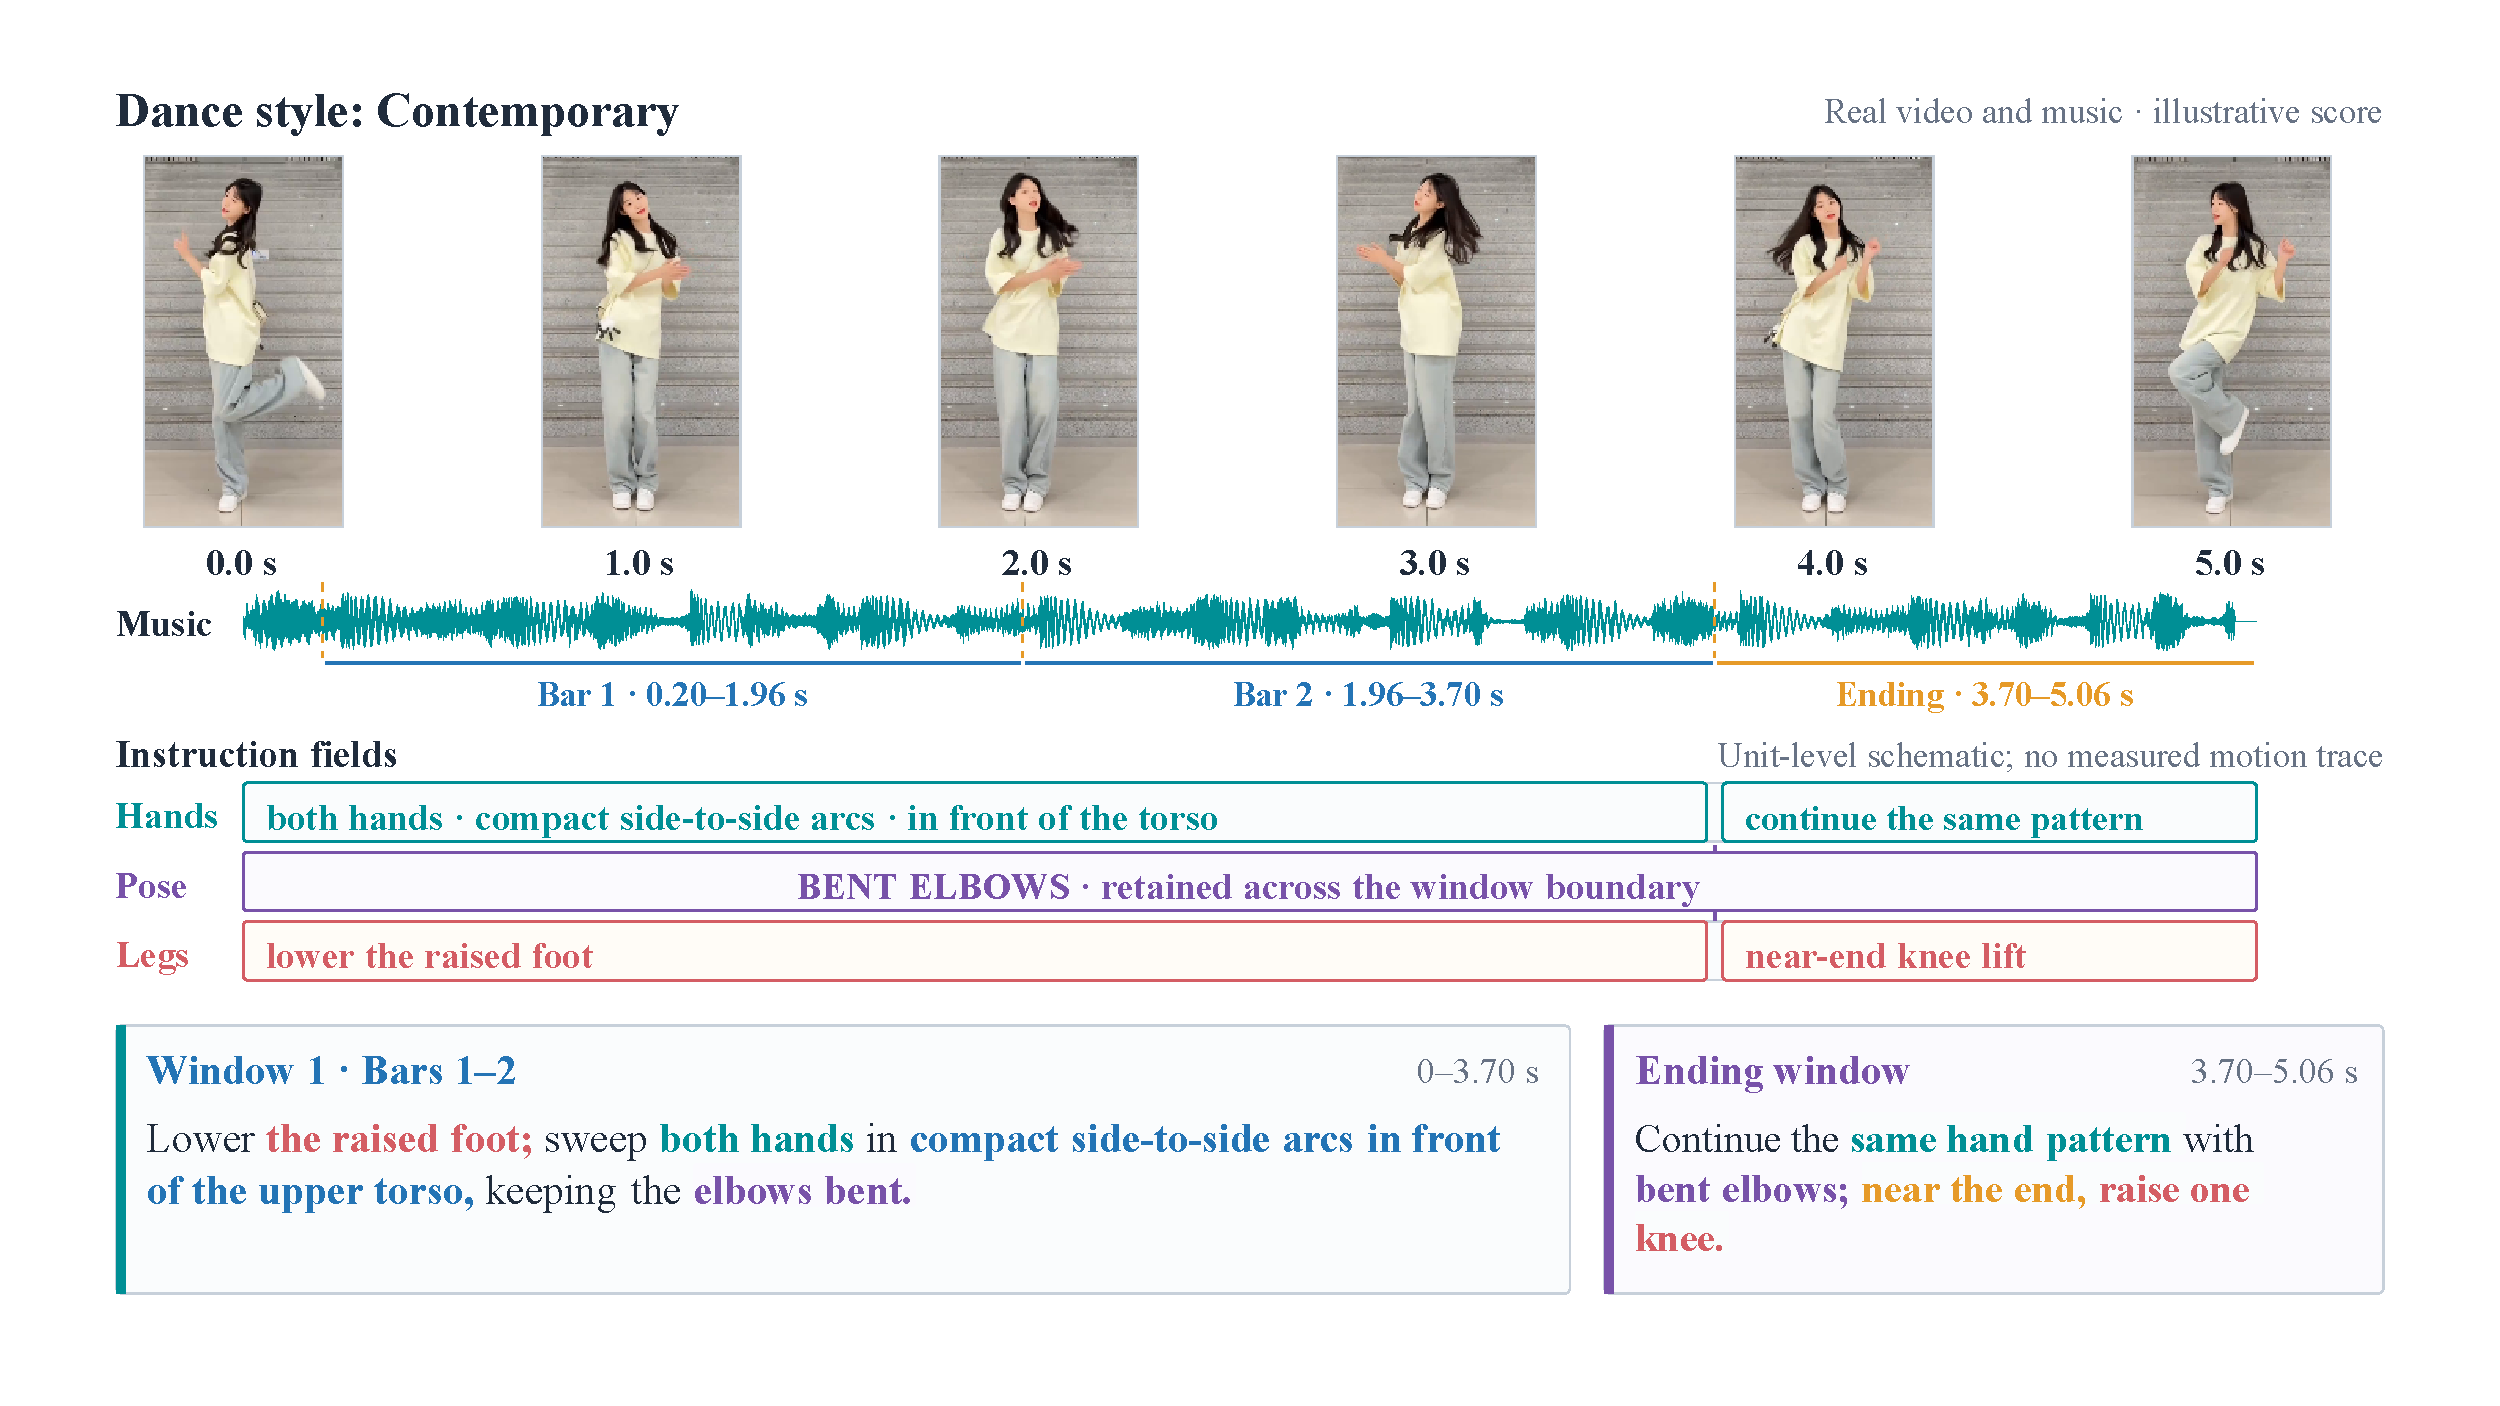
\includegraphics[width=\textwidth]{figures/revision_20261117_v3/paper/choreography_case.pdf}
\caption{\textbf{What makes a movement description informative.}
Six equally spaced real frames share a clock with the measured music
waveform. Unit-level fields expose body references, movement range and
direction, and the retained elbow state; matching colors connect these
fields to the instructions below. Predicted bars form a two-bar unit and
an ending fragment, with the initial 0--0.20\,s fragment merged.
The authored instructions and field bands illustrate the representation,
not scored predictions, measured action durations, or verified synchronization.}
\label{fig:choreography-example}
\end{figure*}
